%\documentclass{nature}
\documentclass{article}
\usepackage[english,american]{babel}
\usepackage[backend=biber,style=nature]{biblatex}
\usepackage{todonotes}
\usepackage{subfiles}
\usepackage{grffile}
\usepackage{booktabs}
\usepackage{hyperref}
\usepackage{graphicx}
\usepackage{fullpage}
\usepackage{algorithm}
\usepackage{algorithmic}
\usepackage{amsmath}
\usepackage{subcaption}
\usepackage{multicol}

\renewcommand{\vec}[1]{\mathbf{#1}}


\addbibresource{connectomics motif.bib}
\addbibresource{connectomics motif-relational models.bib}

\DeclareGraphicsRule{.ai}{pdf}{.ai}{}


\title{Discovering cell type motifs in connectomics data}
\author{Eric Jonas, Konrad Kording}

\begin{document}
\maketitle

\todo{Citations}
\todo{Log score plots for real data} 
\todo{Hierarhcical structure?}
% \begin{affiliations}
%   \item Something Something
%   \item Something Something
% \end{affiliations}

\begin{abstract}
  New techniques produce massive data about neural connectivity,
  necessitating new analysis methods to discover underlying
  structure. There is strong evidence for microcircuitry, where the
  probability of connections depends on the types of pre- and
  post-synaptic neurons and their distance. Here we developed a
  nonparametric Bayesian technique that identifies neuron type and circuitry
  patterns from the connection data. We show that the approach recovers
  known neuron types in the retina, reveals interesting structure in
  the nervous system of c. elegans, and automatically discovers the
  structure of microprocessors. Our approach is a first step towards
  condensing connectomics data into meaningful, human readable
  structure.
\end{abstract}

\section*{Introduction}
Emerging techniques \autocite{Lichtman, Zador, Denk} promise to
quantify the location of each neuron within a volume of interest,
along with its connections to all other neurons. Far exceeding the
capacity of neuroanatomists to trace small circuits, this leads to
enormous datasets that quantify aspects of the nervous system. The
rise of high-throughput sequencing techniques necessitated the
development of novel computational methods to understand genomic
structure, ushering in an era of bioinformatics as an independent
discipline \autocite{}.

The brain consists of multiple kinds of neurons, each of which is
hypothesized to have a specific role in the overall
computation. Neuron types differ in many ways, e.g. chemical or
morphological, but they also differ in the way they connect to one
another. In fact, the idea of well defined local connectivity patterns
has been prominent in many areas, ranging from sensory (e.g. retina,
\autocite{} via processing (e.g. neocortex) to movement (e.g. spinal
cord) \autocite{}. Indeed, such repeated patterns also exists in
human-made computing circuits. It remains an important challenge to
develop algorithms to use anatomical data, e.g. connectomics, to back
out underlying connectivity motifs.

The discovery of structure is a crucial aspect of network
science. Early approaches focused on global graph properties, such as
the types of scaling present in the network \autocite
{WattsStrogatz1998} .  While this approach leads to an understanding
of global network, more recent work aims at identifying small-scale
repeat patterns, or “motifs” in networks. \todo{There's the
  Science2002 paper by Milo et. al. that explicitly looks at 'motifs'}
A motif is a set of nodes with conserved relations that appears
multiple times in a network, for example a set of three nodes that are
each connected to one another. 

When it comes to neuroscience, we might
expect that a motif consists of the kinds of cells that jointly make
up a microcircuit along with their distance and cell-type dependent
connectivity. The same motif should then appear in multiple locations
in the nervous system. Combining motif-discovery ideas with specific
knowledge about the kinds of motifs in the nervous system promises
better structure discovery.

The discovery of structure in probabilistic graphs is a crucial aspect
in machine learning. Commonly used algorithms include spectral methods
\autocite{},   community-based-detection   methods  \autocite{},   and
stochastic block  models \autocite{NowickiSnijdders2001}.  While these
approaches powerfully  incorporate the probabilistic nature of neural
connections \autocite{} they do not generally consider the known fact
that  the  probability  of  connections  between  neurons  depends  on
distance. Combining such probabilistic models with a spatial component
to model distance promises to  improve the detection of microcircuitry
from neural data.

Here we describe a Bayesian non-parametric model that can discover
circuit structure automatically from connectomics data: both the cell
types and their spatial patterns of interconnection. We apply it to
three computing systems: the mouse retina connectome \autocite{}, the
c. elegans connectome \autocite{}, and a ``connectome'' of a classical
microprocessor. In all cases, we discover cell-type to cell-type
connectivity that depends on spatial distance and these connectivity
functions depend on the two involved cell types. Comparing the cell
types discovered by the algorithms with those obtained by anatomists
based on orthogonal information reveals a high degree of agreement. We
present a scalable approach to infer microcircuitry from connectivity
data.

\begin{figure}
  \centering 
    \centerline{\includegraphics[width=183mm]{overview.ai}}
  \caption{An overview of our method. a. Input data is
an adjacency matrix indicating whether cell $i$ (row)
synapses on cell $j$ (column). The location of each cell in space is known. 
b. Our algorithm discovers hidden cell types in this connectivity data
by assuming all cells of a type share a distance-dependent connectivity 
profile, c.), with cells of other types. This results in a clustering 
of the cells by those hidden types. b.) shows the cell adjacency
matrix with cells of the same type grouped together. d.) shows
the learned probability of connection between our different types
at various distances, illustrating short-range and long-range
connectivtiy patterns.}

\end{figure}

\section{Results}
We use a Bayesian structure discovery approach that is based on
assumptions about the way positions and cell types affect the
probability of connections between cells, a so-called generative
model. The probability of connections between pairs of neurons
decreases with distance, but how high the baseline probability of
connection is and how quickly it decays with distance depends on the
two cell-types. We combine annealing with Markov Chain Monte Carlo to
perform simultaneously joint posterior inference over the structure,
parameters, and hyperparameters of the model. This procedure yields a
division of all neurons into cell-types along with the distance and
type dependent connectivity probabilities. These results can then be
compared with the results of previous anatomical studies that have
used other aspects of neurons, such as chemical properties and
cell-morphology to divide neurons into types.

Before we can use a probabilistic model to analyze real data we first
need to assess if the model works properly. We thus started out by
simulating data for which we know the correct structure and comparing
the estimated structure based on the algorithm (see methods) with the
one we used for simulation. We find that the model does a good job of
recovering the structure we used to generate the data (Fig
1A). Indeed, it does far better than a simpler and well established
model (stochastic block) that assumes that there is no distance
dependence to the connectivity. The model converges relatively
quickly, which is enabled by xxx cool tricks we used to speed it
up. It appears that the model behaves the way it should and allows
application to large datasets.

\begin{figure}
  \centering 
  \centerline{\includegraphics{synthetic.ai}}
  \caption{Correct recovery of true numbers of hidden classes
in synthetic data. a.) Other models overcluster the number
of classes as they fail to take distance into account, whereas
our model finds close to the true number of classes. b.) ARI, a measure
of ``correct clustering'', for
different true class counts, between our model and a traditional
nonparametric stochastic block model. c.) Multiple Markov chains iterateively
converge towards a highly-probable solution. }

\end{figure}

\subsubsection{Mouse Retina}
The retina of the mouse \autocite{Masland2001} is an example where we
should expect to have connectivity patterns that are well approximated
by our generative model. It is known that there are multiple classes
of cells that can be grouped into ganglion cells that transmit
information to the rest of the brain, bipolar cells that connect
between different cells, and amacrine cells that feed into the
ganglion cells (cite some review). Recent research \autocite{Helmstaedter2013} has
produced a large dataset containing both the types of cells from
orthogonal approaches, and also the connectivity matrix between all
reconstructed cells. We want to know to which level we can classify
neurons into types based on this connectivity only.

The algorithm took 8 hours to converge to a locally optimal solution,
dividing neurons into a set of cell types (Fig 2a). For each pair of
neurons there is a specific distance dependent connection probability
(Fig 2b), which is well approximated by the model fit. Moreover, each
type of cell is rather isotropically distributed across space (Fig 2c)
as should be expected for true cell types. The algorithm is thus able
to extract meaningful structure from the data.

Comparing the results of the algorithm to other information sources
allows evaluating the quality of the type determination. We find that
the types tend to reflect the known laminar distribution in the retina
(Fig 2a, outer ring), which is exciting as the algorithm did not
actually use this type of information. Moreover, we can compare the
results from our algorithm with cell-type determinations by
professional anatomists, who distinguish between 71 types of
neurons. The algorithm yields a separation of neurons into a smaller
number of types that are, however, highly correlated with those of the
anatomists.

Our types closely reflect the (human-determined) segmentation of cells
into retinal ganglion, narrow amacrine, medium/wide amacrine, and
bipolar cells (Figure 2a, outermost ring). [TODO: Do we actually
assign any of the unknown cells correctly? are types 72-79 “differet”
or simply unknown?]


\begin{figure}
  \centering 
  \centerline{\includegraphics{mouseretina.ai}}
  \caption{Discovering cell classes in the mouse retina connectome. 
a.) Input adajacency data for 950 cells for which soma positions were known. b. clsutered adjacency matrix. c.) connectivity diagram showing our clusters, as
well as the cell depth and known cell type of each cell. Our model agrees
with the cell types traditionally identified by anatomists, and identifies 
laminar-specific connectivity patterns. d.) Connectivity between our
clusters as a function of distance -- the cluster consisting primarially of
retinal ganglion cells (lower left-center) exhibits the expected near and
far connectivity.}
\end{figure}

\subsection{C. elegans}

The roundworm Caenorhabditis elegans is a model system in
developmental neuroscience\autocite{White1986}, with the location and
connectivity of each of 302 neurons deterministically known. This
incredible cross-organism consistency led to early mapping of the
c. elegans chemical and electrical (gap junction) connectome. Unlike
the retina, only the motor neurons in c. elegans exhibit regular
distribution in space, as they follow the body axis. Most interneurons
are concentrated in various ganglia that project throughout the entire
animal, and the sensory neurons are primarily located in the animal
head.

Using both the chemical and electrical connectivity (see methods), we
determined the underlying clusters explained by connectivity and
distance (fig ba). A superficial inspection of the results shows
clustering into groups consisting roughly homogeneously of motor
neurons, sensory neurons, and interneurons. Closer examination reveals
agreement with the classifications originally outlined by Brenner in
1986.  [create structure that mirrors the mouse retina paragraphs]

[start paragraph with summary sentence] Motorneuron types AS, DA, and
VA, all exclusively postsynaptic, are clustered together, as are
motorneuron types VD and DD. VC, DB, and VB also mostly share a
cluster. Various head motor neurons, including classes SMD, RMD, and
RIM are clustered together. Interneurons with known
anatomically-distinct connectivity patterns, such as RIA (2 cells) or
AVA (2 cells) are clustered into pure groups. The algorithm even
correctly places the single-cell class DVB in a distinct group. Note
our clustering does not perfectly recover known groupings -- several
combinations of head and sensory neurons are combined, and a
difficult-to-explain group of 2 VD, 2 VB, a VA, and a DD neuron are
grouped together. [algorithm recovers surprising structure based
merely on connectivity even though only 278 cells and not spatially
homogeneous]


\begin{figure}
  \centering 
  \centerline{\includegraphics{celegans.ai}}
  \caption{Discovering cell classes in the \textit{c. elegans}
    connectome. a.) Initial cell connectivity matrix, red are
    (directional) chemical synapses, blue are electrical
    synapses. Point size is proportaionl to synapse count between
    those cells. b.) Clustered adjaceny matrix showing identified
    clusters. c.) Inter-cluster connectivity, showing the position of
    each cell along the body axis as well as the ``true'' cell type --
    both coarse (motor, sensory, and interneuron) as well as fine
    (small text labels). }
\end{figure}

\subsection{Microprocessor}

To show the applicability of our method to other connectome-style
datasets, we obtained the spatial location and interconnectivity of a
transistors in a classic microprocessor, the MOS Technology 6502 (used
in the Apple II) \autocite{datasource}. We identified a region of the
processor with complex but known structure containing the primary
general-purpose registers X, Y, and S (figure). Computer architects
use common patterns of transistors when designing circuits, 
with each transistor having a ``type'' in the circuit. 


Our algorithm identifies areas of spatial homogeneity that mirror the
kown structure in the underlying architectural circuit, segementing
transistor groups. One group contains the ``clocked'' transistors,
one group with their source connected to ground, and one with their
drain connected to ground. The repeat patterns of spatial connectivity
are visible in figure~\ref{fig:microprocessor}a, 

\begin{figure}
  \centering 
  \centerline{\includegraphics{mos6502.ai}}
  \caption{Microprocessor data}
\end{figure}


\section{Discussion}
We have presented a machine learning technique that allows cell types
and connectivity structure to be discovered using only spatial and
connectivity data. We have shown its applicability to a newly
published connectomics dataset from the mouse retina, the classical
connectivity of the worm c elegans, and the connectivity of a
historical man-made microprocessor. We have found that spatial
connectivity alone is sufficient to discover interesting motifs that
were known to exist in the systems based on decades of previous
research which had utilized extensive additional information. “

For probabilistic models like ours, no known solution exists to
exactly find the most probable parsing of the neurons into cell-types
and connectivity patterns . We employ a collection of Markov-chain
Monte carlo techniques [reference methods] but while different
initializations converge to similar ultimate values, we can never
realistically obtain the global optimum. There are a broad range of
techniques that may offer better approximations to the global optimum
\autocite{Wanga2012,FritzJonathan} and future work could adapt them to
the problem we addressed here.

Our inference becomes slower as the amount of data increases. Our
algorithm required 10xxx hours for 1000 neurons and would therefore
take months for 10,000 neurons, which would not be acceptable. Various
new techniques promise to allow similar calculations to take less time
and scale to larger datasets \autocite{}.


*Fixed and hand selected likelihood link functions We picked the
sigmoid. Should be estimated, Our small collection of parametric forms
for spatial functions are obviously not exhaustive

*We do not use other sources of information that are totally there in
the datasets. Cell morphology could be used. Laminar organization.

*Larger datasets will generally allow algorithms to distinguish more
distinct types (cite supplemental data) and more data should
algorithms to get closer to the results from anatomy. Moreover, in
general, for such problems precision increases with the size of the
dataset and the 9xxx cells that we have are not sufficient to
statistically distinguish all the cell types known in anatomy
(71xxx). Still, using only connectivity it is possible to meaningfully
divide neurons into classes.

[ how this changes things] There exist a range of previous approaches
to the discovery of microcircuitry [coherence of language]
(cites). These generally involve a great deal of manual labor and
ad-hoc determination of what constitutes a “type” of cell -- to this
day there are disagreements in the literature as to the “true” types
in the mammalian retina. Much as phylogenomics has changed our
understanding of animal ontologies, modern large scale data will allow
the efficient unbiased discovery of structure. The sheer amount of
available data demands the introduction of algorithmic approaches.


*A new way of phenotyping, combining spatial motif ideas with clustering ideas

*Novel data analysis techniques are required to lead us into the big
data age. Our approach is orthogonal to all others (because in high d
everything is orthogonal).

Ultimately, we will need to combine information across different
sources into a joint understanding of neural function. Distinct cell
types differ in morphology, connectivity, transcriptomics, relation to
behavior or stimuli and many other ways. Algorithms based on each type
information can then be combined to synthesize all the available
information from one experiment or even across experiments into a
joint model of brain function.


\section{Methods}
\section{Methods Summary}

% this should clearly describe the inputs

% the outputs 

% the model 


We assume as input a connectivity matrix $R$ defining the connections
between cells, as well as a distance function $d(e_i, e_j)$
representing a (physical) distance between adjacent cells. See the
supplemental material for extension to multiple connectivity
matrices. We assume there exist an unknown number of latent
(unobserved) cell types, $k$, $k \in \{1, 2, 3, \dots\}$, and that
each cell $e_i$ belongs to a single cell type, $c_i = k$. The observed
connectivity between two cells $R(e_i, e_j)$ then only depends on
their latent type and their distance through a link function $f(c_i,
c_j, d(e_i, e_j))$ If $c_i=m$ and $c_j=n$ then there exists a
latent-class-specific set of parameters $\eta_{mn}$ which parametrizes
$f$, as well as a set of global hyper parameters $\theta$.

We then jointly compute the maximum a posteriroi (MAP) estimate of the
class assignment vector ${c_i}$, the parameter matrix $\eta_{mn}$, and
the global model hyperparameters $\theta$ :

\begin{equation}
  p(\vec{c}, \eta, \theta | R ) \propto \prod_{i, j} p(R(e_i, e_j) | f(d(e_i, e_j) | \eta_{c_ic_j}), \theta) \prod_{m, n} p(\eta_{mn} | \theta)  p(\theta) p(\vec{c} | \alpha) p(\alpha) p(\theta)
\end{equation}


% Methods section 3000 words
% methods summary does not appear in the online text
% methods section can have no figures or tables [grrr]
% todo describe multiple independent relations? 

\subsection{Probabilistic Model}

Our model is a extension of infinite stochastic block models
\autocite{Kemp2006a,Xu2006} to incorporate spatial constraints.

\todo{infinite subset relaitonal model has good summaries}

We describe three link functions, ``Logistic-distance Bernoulli'',
``logistic-distance fixed-lambda Bernoulli'', and ``logistid-Distance
Poisson''. 

The ``logistic-distance Bernoulli'' model associates with each latent class 
two parameters, $\mu_{mn}$ and $\lambda_{mn}$, and the probability that two
cells $e_i$ and $e_j$ are connected is given by
\begin{eqnarray}
p^* &=& \frac{1.0}{1 + \exp \frac{d(e_i, e_j) - \mu_{mn}}{\lambda_{mn}}}\\
p &= & p^* \cdot (p_{max} - p_{min}) + p_{min}
\end{eqnarray}
where $p_{max}$ and $p_{min}$ are per-graph hyperparameters. Per-component parameters $\mu_{mn} \sim \exp(\mu | \mu^{hp})$ and $\lambda_{mn} \sim \exp(\lambda | \lambda^{hp})$. 
Inference is performed on these hyperparameters as well, see TODO supplemental 
for details. 

We use a Dirichlet-process prior on cluster assignments, which allows
the number of clusters to be determined automatically. In brief, the
probability of a cell belonging to a cluster is proportional to the
number of datapoints already in that cluster, $m_k$, such that $p(c_i
= k) \propto \frac{m_k}{N + \alpha}$ and the probability of the cell
belonging to a new cluster $k'$ is $p(c_i = k') \propto
\frac{\alpha}{N + \alpha}$.


\subsection{Inference} 
We perform posterior inference via Markov-chain Monte Carlo (MCMC),
annealing on the global likelihood during the traditional burn-in
phase. MCMC transition kernels for different parts of the state space
can be chained together to construct a kernel whose ergodic
distribution is the target ergodic distribution over the entire state space. 

Our first transition kernel (``structural'') performs gibbs sampling 
of the assignment vector $p(\vec{c} | \eta, \theta, \alpha)$. 
The lack of conjugacy in our likelihood model makes an explicit 
evaluation of the conditional assignment probabilities impossible, 
motivating us to use an auxiliary variable method \autocite{Neal2000}
in which a collection of ephemeral clusters are explicitly represented
for the duration of the Gibbs scan. 

We then employ a transition kernel to update the per-component
parameter values $\eta_{mn}$. Conditioned on the assignment vector
$\vec{c}$ and the model hyperparameters $\theta, \alpha$ the 
individual $\eta_{mn}$ are indepednent. We slice sample \autocite{Neal2003}
each component's parameters, choosing the slice width as a function
of the global hyperparameter range. 

The global hyper-parameters, both $\alpha$ and $\theta$, are allowed
to take on a discrete set of possible values. As $\theta$ is often a
tuple of possible values, we explore the cartesian product of all
possible values. We then Gibbs sample, which is always possible in a 
small, finite discrete state space. 

We chain these three kernels together, and then globally
anneal on the likelihood from a temperature of $T=64$ down to 
$T=1$ over 300 iterations unless otherwise indicated, and
then run the chain for another $100$ iterations. 

To pick the MAP, we run up to $100$ simultaneous chains in parallel,
iniitalized from different random initial points in the statespace,
and then pick the chain with the highest log likelihood. Early
experiments attempted to use the full ensemble of chains as an
estimate of the posterior but were abandoned due to the difficulty of
summarizing the posterior over such a complex state space, whcih is an
ongoing area of research in the probabilistic modeling community
\autocite{}.


\subsection{Validation}


\subsection {Mouse Retina}
Dense serial electron microscopy of a $VOLUMNE$ in the mouse retina by
\autocite{Helmstaedter2013} yielded a listing of places where neurons
come into contact. There were $number$ cells originally, and selected
the $950$ for which the location of the soma could be reconstruted
from the provided cell plots (soma locations were not provided by the
study's authors in machine-readble form). Ultimately
this left a matrix between the total synapse-like contact area between
all pairs of 950 cells. Area was thresholded at $0.5\mu m$, determined
by hand, to yield a 950 $\times$ 950 entry matrix that served as input
to our algorithm. We measured the distance between cells using
the reconstructed soma centers, and used the Logistic-Distance
spatial relation. Hyperprior distributions are shown in \ref{supplemental}. 

\subsection{C. elegans}

We obtained the connectome of c. elegans from \autocite, and isolated
the 279 nonpharyngeal neurons, with a total of 6393 chemical synapses
and 890 gap junctions originally cleaned up in \autocite{Chen2006}. A
cell's position was its distance along the anterior-posterior axis
normalzed between zero and one. We used both networks, the chemical
network as a directed graph and the electrical network as undirected
graph. We use the synapse counts with the logistic-distance poisson
likelihood, scaling the counts by a factor of 4 to compensate for 
the Poisson's overdispersion. 

\subsection{Microprocessor}
We extracted the connection graph for all transistors in the MOS6502
\autocite{visual6502}. Each transistor has three terminals: an input
G, a source, and a drain, labeled C1 and C2. We identified the region
consisting of the three general-purpose registers X, Y, and S via
visual inspection and focused our efforts there. We created a total of
six connectivity matrices by examining possible terminal parings. One
graph, for example, $R^{gc_1}(e_i, e_j)=1$ if transistor $e_j$ and $e_j$ are
connected via pins $g$ and $c_1$. 
\todo{How do we handle symmetry here?}

% \begin{addendum}
%  \item Put acknowledgements here.
%  \item[Competing Interests] The authors declare that they have no
% competing financial interests.
%  \item[Correspondence] Correspondence and requests for materials
% should be addressed to A.B.C.~(email: myaddress@nowhere.edu).
% \end{addendum}
\section{Supplemental}
\subsection{Source code}
\todo{Put up website}

All source code and materials for running experiments can be
obtained from the project website, at http://spatialrelation.github.io. 

\subsection{Extension to multiple graphs}
The model can handle multiple graphs $R^q$ simultaneously with a shared clustering by simply considering the product of 
\begin{equation}
  p(\vec{c}, \{\eta^q\}, \{\theta^q\} | \{R^q\} ) \propto \prod_q \Bigg(\prod_{i, j} p(R^q(e_i, e_j) | f(d(e_i, e_j) | \eta^q_{c_ic_j}), \theta^q) \prod_{m, n} p(\eta^q_{mn} | \theta^q)  p(\theta^q) \Bigg) p(\vec{c} | \alpha) p(\alpha) 
\end{equation}

\subsection{Microprocessor Netlist annotation}
\begin{figure}
  \centering 
    \centerline{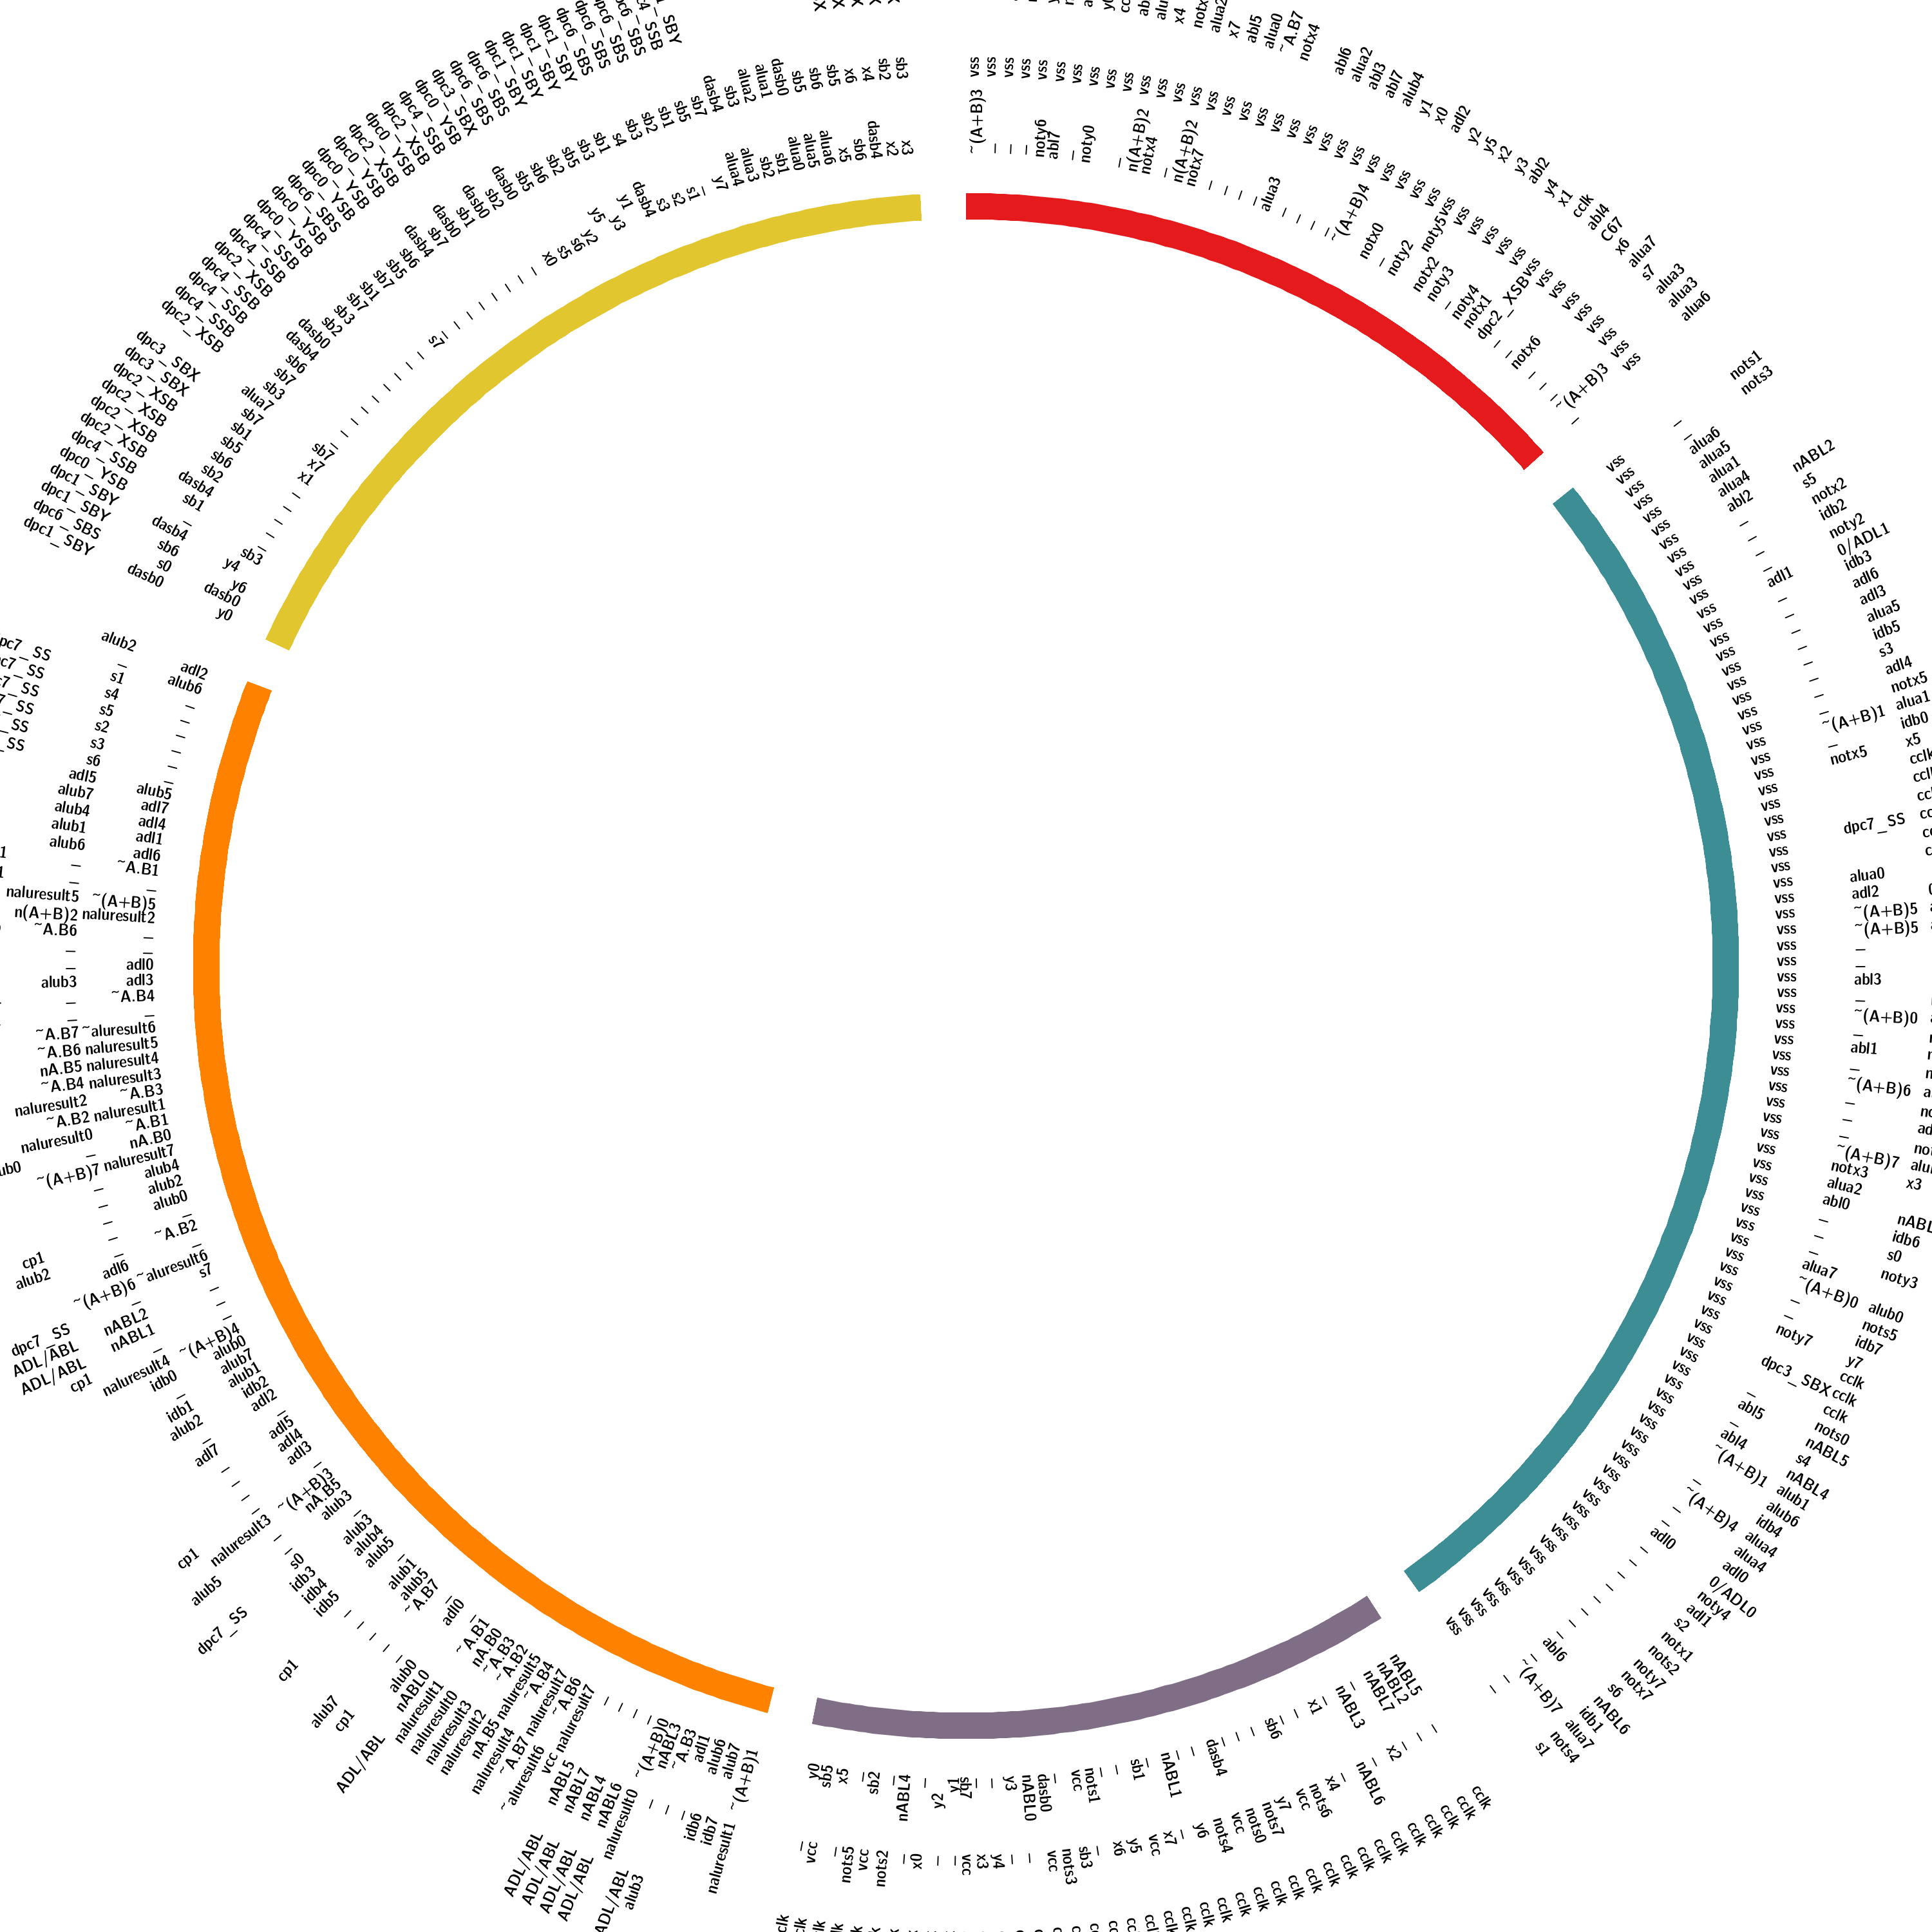
\includegraphics[width=183mm]{mos6502/sixrelation.xysregs.ldfl.circos.4.R2.ai}}
\end{figure}

\subsection{Hyperprior grids}

For the mouse retina Logistic-Distance Bernoulli model, we gridded $\mu^{hp}$ and $\lambda^{hp}$ into 40 $\log_{10}$-spaced points 1.0 and 80. $p_{min} \in [0.001, 0.005, 0.01]$ and $p_{max} \in [0.80, 0.90, 0.95, 0.99$.

For the c. elegans data with the Logistic Distance poisson model, we gridded $\mu_{hp$ and $\lambda$ into 20 $\log_{10}$-spaced points bween 0.2 and 2.0, and the $ratescale^{hp}$ parameter into 20 $\log_{10}$-spaced points between 2.0 and 20.0. We globally set $rate_{min}=0.01$. 

\todo{Explain Adjusted Rand Index} 

\printbibliography

\end{document}

